\section{Results}
\label{sec:results}

\subsection{A native band recovers most of the two-scale context gap}
\label{sec:dense_result}

\begin{figure*}[t]
  \centering
  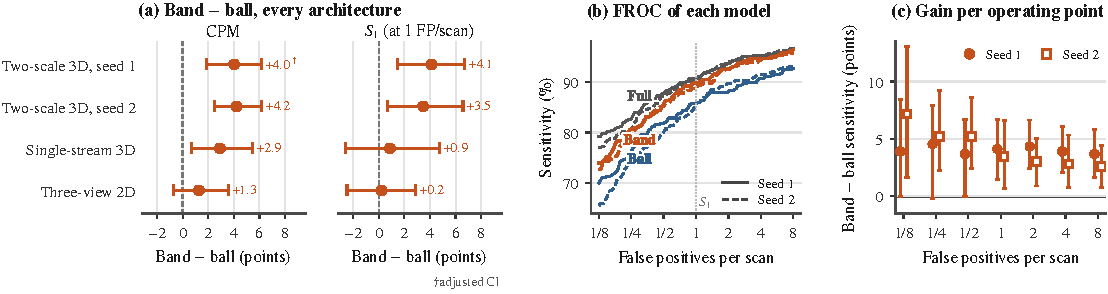
\includegraphics[width=\textwidth]{figures/restoration.pdf}
  \caption{Restoring the band improves two separately fitted two-scale 3D rankers on the same \EvalScans{} scans. A shows paired effects on CPM and sensitivity at matched 1 FP/scan. The primary CPM bar is adjusted across three locked comparisons. Other bars give pointwise 95\% patient intervals. B shows matched FROC for ball, ball plus band and full access, using both seeds. The band recovers \PrimaryRecovery\% and \RepeatRecovery\% of the observed full-minus-ball CPM gaps.}
  \label{fig:restoration}
\end{figure*}
\begin{table*}[t]
\centering
\small
\caption{Visibility on 353 reused scans. Absolute CPM is in percent. Paired band-minus-ball effects are in points. $^\dagger$ denotes the primary CPM interval adjusted across three locked contrasts. Other intervals are pointwise 95\%. Recovery is the band gain divided by the observed full-minus-ball CPM gap for each fit.}
\label{tab:visibility}
\begin{tabular}{@{}lrrrrrr@{}}
\toprule
Fitted architecture & Ball & Ball + band & Full & $\Delta$ CPM & $\Delta S_1$ & Recovery \\
\midrule
Two-scale 3D (3691) & 83.58 & 87.60 & 89.37 & $+4.03\,[1.85,\,6.17]$$^\dagger$ & $+4.12\,[1.45,\,6.71]$ & 70\% \\
Two-scale 3D (9143) & 82.83 & 87.05 & 88.63 & $+4.21\,[2.51,\,6.17]$ & $+3.47\,[0.67,\,6.59]$ & 73\% \\
Single-stream 3D (3691) & 80.94 & 83.85 & 85.84 & $+2.91\,[0.69,\,5.48]$ & $+0.87\,[-2.59,\,4.73]$ & 59\% \\
Three-view 2D (9143) & 81.28 & 82.55 & 84.75 & $+1.27\,[-0.71,\,3.58]$ & $+0.22\,[-2.49,\,2.88]$ & 37\% \\
\bottomrule
\end{tabular}
\end{table*}


The primary two-scale ranker achieves \BallCpm\% CPM with the native ball, \BandCpm\% with the ball and band, and \FullCpm\% with the full field (Fig.~\ref{fig:restoration} and Tab.~\ref{tab:visibility}). Restoring the band raises CPM by \RestorePrimary{} points under the three-contrast adjustment. The pointwise interval is \RestorePrimaryPointwise{} points. The second seed yields \RestoreRepeat{} points, using a pointwise interval. Matched $S_1$ gains are \RestoreOne{} and \RepeatOne{} points. All effects are calculated before rounding the absolute scores.

The absolute ranking curves separate across operating points, with higher sensitivity under restored access at all seven release rates in both fits. The gain represents \PrimaryRecovery\% and \RepeatRecovery\% of the observed gap from ball to full CPM. It leaves a residual advantage for the full crop. The recovery fraction refers to fitted ranking performance at the same proposals. It depends on the architecture, the training procedure and the operating points used in CPM. The band gains remain positive in each reused subset group and essentially unchanged when all marks are eligible. Supplement Sec.~S3 reports all seven operating points and the uncapped comparisons.

The independent-cutoff analysis separates a change in ranking from threshold calibration. Transferring each model's threshold selected on the 88 calibration scans changes sensitivity by \TransferredPrimary{} points for the primary fit and \TransferredRepeat{} points for the second. The achieved FP burdens differ by model. The two matched results therefore give stronger evidence for ranking improvement at 1 FP/scan than the fixed-threshold results give for deployment at a particular burden.

\subsection{Native source coverage matters at the same image entry point}
\label{sec:source_result}

\begin{figure*}[t]
  \centering
  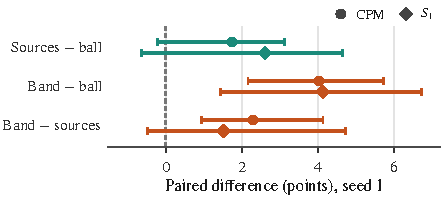
\includegraphics[width=\textwidth]{figures/coverage.pdf}
  \caption{Native query sources and the dense band enter the same image encoder. A counts distinct retained exterior native voxels per proposal that can contribute to the centered crop, averaged over the full evaluation stream. B gives paired CPM effects for the same two-scale 3D architecture and seed. All bars in B are pointwise 95\% patient intervals. The dense band outperforms exact query-source access even when both enter at the first image layer.}
  \label{fig:coverage}
\end{figure*}

A late residual could underperform simply because it receives sparse information after the image features have been computed. The native-source arm removes that difference in processing between the two image inputs. It retains the ball and the union of positive-weight sources of the same 384 query locations. Both this arm and the dense-band arm can learn spatial filters over all visible intensities from their first convolution. The mean exterior coverage reaching the centered crop is \QuerySources{} native sources per proposal in the query-source arm and \BandSources{} in the dense-band arm (Fig.~\ref{fig:coverage}).

Giving the encoder the query sources changes CPM over the ball by \SourcesGain{} points in the primary seed. The band adds a further \CoverageGap{} points over those sources. The point estimate for the latter comparison is positive in both subset groups, and removing the cap gives the same pooled CPM effect. At matched 1 FP/scan, query-source versus ball is \SourcesOne{} points and band versus query-source is \CoverageOne{} points. The CPM evidence is clearer than the result at that individual operating point.

The residual gap remains when the point of entry and image capacity are matched. It supports a role for the additional coverage and spatial continuity supplied by the dense band under this masking scheme. The holes between the retained query sources can disrupt patterns that a filter would otherwise see across the band. Their effect and that of the additional native measurements are coupled in this intervention. The query-source arm also retains the underlying HU values before sparse interpolation. Its comparison with the late endpoint heads combines changes in representation, fusion and the values available to the ranker.

\subsection{Relative geometry alone leaves a large sparse gap}
\label{sec:spatial_result}

\begin{figure*}[t]
  \centering
  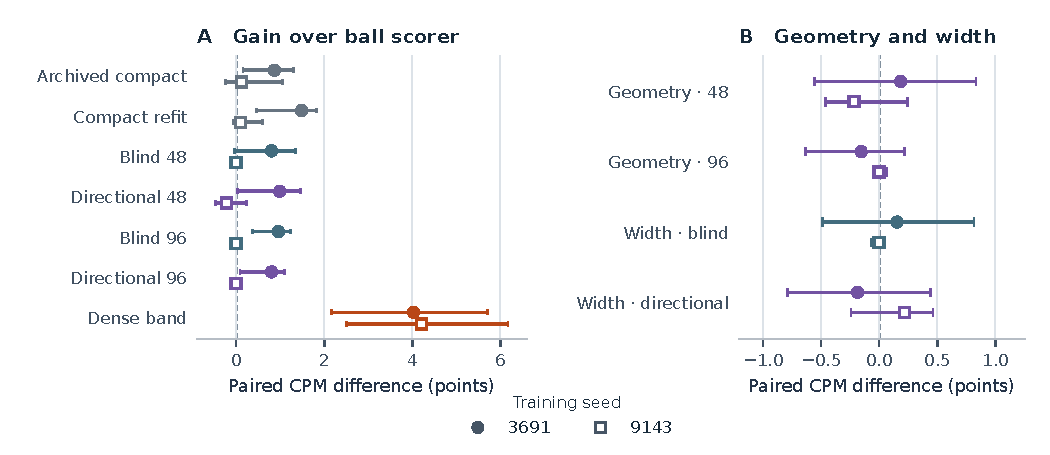
\includegraphics[width=\textwidth]{figures/spatial.pdf}
  \caption{Paired CPM effects of the same 384 readings on the two frozen ball scorers. A compares the archived compact head, its frozen-image refit and both widths of set attention against the same ball-only baseline. Dense restoration is shown on the same scale. B isolates the directional bias at fixed width and the width change at fixed bias. Pointwise 95\% intervals use shared patient draws. The two markers denote separate training seeds.}
  \label{fig:spatial}
\end{figure*}

Sparsity alone does not require pooling away angular structure. We test its value by adding relative directions to an otherwise identical attention head. The model can use line neighborhoods without relying on absolute orientation or learning a positional code from the ordering of the array. At width 48 the directional-minus-blind CPM effects are \GeometrySmallPrimary{} and \GeometrySmallRepeat{} points across the two seeds. At width 96 they are \GeometryLargePrimary{} and \GeometryLargeRepeat{} points. The matched $S_1$ differences also provide little evidence of a gain (supplement Sec.~S4). Doubling the width yields no consistent improvement in either geometry condition (Fig.~\ref{fig:spatial}B).

The compact refit changes CPM relative to the archived compact fit by \RefitPrimary{} and \RefitRepeat{} points. All refits share frozen image logits and the same sampling procedure. The primary compact refit gives the largest observed sparse gain over its ball scorer among the tested readouts for that seed. The dense band still leads the compact refits by \CompactGapPrimary{} and \CompactGapRepeat{} CPM points. The directional width-48 head trails the dense band by \ResidualSmallPrimary{} and \ResidualSmallRepeat{} CPM points and by \ResidualSmallOnePrimary{} and \ResidualSmallOneRepeat{} matched sensitivity points at 1 FP/scan. The width-96 comparison gives CPM gaps of \ResidualLargePrimary{} and \ResidualLargeRepeat{} points. These differences refer to the fitted readouts and use their unchanged ball-only references.

Taken together with the same-encoder source comparison, the attention experiments narrow the explanation. Giving a late readout the relative directions of the sampled axes, increasing its width and fitting after the image encoder converges leave a substantial CPM difference from dense access. The same backbone also benefits from denser access when all exterior evidence arrives before the first convolution. A more informative sampling pattern or a different geometry-preserving fusion could still use the existing budget of readings differently.

\subsection{The largest gains occur where the band reaches a lesion}
\label{sec:anatomy_result}

\begin{figure*}[t]
  \centering
  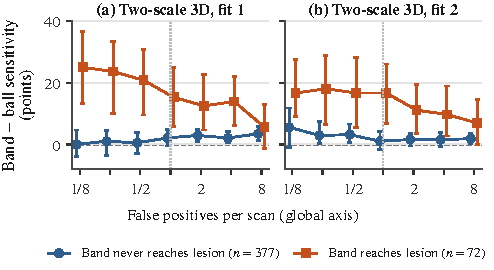
\includegraphics[width=\textwidth]{figures/anatomy.pdf}
  \caption{Anatomy groups defined from all original matching proposals before scores were joined. Sensitivity differences compare band and ball at global FP/scan targets on the complete streams. A lesion is in the overlap group if the band of any matching proposal reaches its majority-reader contour. The 377 never-overlap and 72 overlap lesions are shown, with paired pointwise 95\% patient intervals. The full FROC still includes the six unlinked lesions and the six linked lesions without proposals.}
  \label{fig:anatomy}
\end{figure*}
\begin{table*}[t]
\centering
\small
\caption{Lesion sensitivity at global 1 FP/scan, with a separate FROC curve for each model. All 461 lesions and all evaluated false marks contribute to the global curves. Effects are paired, with pointwise 95\% intervals.}
\label{tab:anatomy_one}
\begin{tabular}{@{}llrrrr@{}}
\toprule
Seed & Group & $n$ & Ball & Band & $\Delta S_1$ \\
\midrule
3691 & Never overlaps & 377 & 89.92 & 92.04 & $+2.12\,[-0.52,\,4.79]$ \\
3691 & Any overlap & 72 & 69.44 & 84.72 & $+15.28\,[5.81,\,25.00]$ \\
3691 & Linked, no proposal & 6 & 0.00 & 0.00 & $+0.00\,[0.00,\,0.00]$ \\
3691 & Unlinked & 6 & 100.00 & 100.00 & $+0.00\,[0.00,\,0.00]$ \\
9143 & Never overlaps & 377 & 89.92 & 90.98 & $+1.06\,[-1.68,\,4.27]$ \\
9143 & Any overlap & 72 & 69.44 & 86.11 & $+16.67\,[6.85,\,26.09]$ \\
9143 & Linked, no proposal & 6 & 0.00 & 0.00 & $+0.00\,[0.00,\,0.00]$ \\
9143 & Unlinked & 6 & 100.00 & 100.00 & $+0.00\,[0.00,\,0.00]$ \\
\bottomrule
\end{tabular}
\end{table*}


Of \EvalLesions{} reference lesions, 455 link to usable reader contours and 449 of those also have at least one matching proposal. The centered inference crop's visible band reaches majority-labeled lesion tissue at one or more matching proposals for \AnyOverlap{} of those 449. The other \NeverOverlap{} have no band overlap at any matching proposal. Across the entire pool there are 604 reference--proposal pairs, of which 598 have usable contours and 216 overlap. All six unlinked lesions have a matching proposal. The other six are linked lesions outside the proposal ceiling and remain in the denominator.

At 1 FP/scan, the band improves sensitivity in the overlap group by \AnyPrimary{} and \AnyRepeat{} points. The corresponding effects in the never-overlap group are \NeverPrimary{} and \NeverRepeat{} points. The overlap-minus-never difference in gains is \HeteroPrimary{} points in the primary fit and \HeteroRepeat{} in the second. Thus about one sixth of the reference lesions account for over half of the net increase at this target in each fit. The 8-FP pointwise estimates in the never-overlap group are positive with intervals above zero for both fits, while the estimates at 1 FP/scan are compatible with both small gains and small losses. Figure~\ref{fig:anatomy} shows the full range of operating points.

The median reference diameter is $17.36\mm$ in the overlap group and $5.75\mm$ in the never-overlap group. The overlap group also has more matching proposals per lesion. These properties can influence which lesions survive ranking under different visibility. The anatomy groups are observational, with imperfect contour coverage, and every sensitivity estimate also depends on the model's ranking of false marks. This supports the narrower explanation that the largest gains occur where restored voxels include part of the annotated lesion. It leaves the contribution of extra-lesional patterns to the gains unresolved. In the earlier descriptive decision audit at the primary discrete cutoff, the fitted band adds 28 lesions and loses nine. Of the 28 gained lesions, 12 have a highest-scoring retained mark whose band reaches the contour. The all-proposal grouping above is independent of that choice of mark.

\subsection{Transfer across image architectures}
\label{sec:breadth_result}

The distinct single-stream 3D architecture meets the prespecified 80\% full-visibility development criterion, with \SingleCheck\% and \SingleDev\% CPM on the checkpoint and readout development roles. On the evaluation pool, its band gains \SingleGain{} CPM points and \SingleOne{} points at matched 1 FP/scan (Tab.~\ref{tab:visibility}). Its CPM gain remains positive in both reused subset groups. A 3D model that processes the full field in a single hierarchy therefore also benefits from the intervention on the same proposal stream.

The earlier three-view fit gains \TriGain{} CPM points and \TriOne{} points at matched 1 FP/scan. This comparison is inconclusive. Each view uses a limited stack of central slices, so the same native mask is represented differently within the network. The architecture comparisons cover differences in how the resampled crop is processed while keeping patients and candidate locations fixed. The external eligibility recheck identified no untouched full-scan cohort with a usable reference and defensible evaluation route in the available inventories (supplement Sec.~S1).

\subsection{Compact controls and the full-context increment}
\label{sec:compact_result}

The original sparse factorial gives an adjusted endpoint-versus-scalar effect of \RepresentPrimary{} CPM points at fixed logit fusion. The second seed gives \RepresentRepeat{} points. The adjusted effect of embedding versus logit on the endpoint gain is \FusionPrimary{} points in the primary fit. These intervals and the change of sign across seeds leave the representation and conditioning advantages uncertain under this compact head. Paired-minus-sham CPM changes are \PairShamPrimary{} and \PairShamRepeat{} points, and the unpaired comparison is similarly uncertain. This leaves little evidence for a consistent advantage from the nominated opposing correspondence. Supplement Sec.~S3 gives the complete factorial and separately fitted controls.

Adding the paired head to full context with the selected gray-mean morphology term changes CPM by \PracticalPrimary{} and \PracticalRepeat{} points. Both upper interval endpoints fall below the prespecified $+1$ CPM-point target for the tested addition. That is a more precise statement than the representation and conditioning comparisons allow. Matched $S_1$ changes are \PracticalOne{} and \PracticalRepeatOne{} points. The low-FP noninferiority check clears its prespecified margin for the first fit, with a possible loss beyond the margin at the lowest rate for the second. Supplement Sec.~S3 reports the threshold transfer, sham and morphology comparisons.
